\documentclass{beamer}

% Language and Encoding
\usepackage[utf8]{inputenc}
\usepackage[utf8]{vietnam}
\uselanguage{vietnamese}
\languagepath{vietnamese}
% \usepackage[vietnamese]{babel}

% Beamer Theme and Color Customization
\mode<presentation> {
    \usetheme{CambridgeUS}
    \usecolortheme{rose} % tím
    \setbeamercolor{frametitle}{fg=black}
    \definecolor{CambridgeUSRed}{RGB}{163, 31, 52} % Define CambridgeUS theme red color
    \setbeamercolor{block title}{bg=CambridgeUSRed!90, fg=white} % Block title background red, text white
    \setbeamercolor{block body}{bg=CambridgeUSRed!8, fg=black} % Block body background light red, text black
}

% Packages for Formatting and Features
\usepackage{hyperref}
\usepackage{subcaption}
\usepackage{listings}
\usepackage{media9}
\usepackage{graphicx} % Allows including images
\usepackage{booktabs} % Table formatting
\usepackage{amsmath}
% \usepackage{subfig}
%\usepackage{subcaption}
\usepackage{caption}
\usepackage{wrapfig}
\usepackage{tikz}
\usepackage{animate}
\usepackage{mathtools}
\usepackage{extarrows}
\usepackage{systeme}
\usepackage{commath}
\usepackage{tasks}
\usepackage{array}
\usepackage{multicol}
\usepackage{lipsum}
\usepackage{pifont}
\usepackage{float}
\usepackage{adjustbox}
% \usepackage{enumitem}

% TikZ Libraries
\usetikzlibrary{shapes.geometric, arrows}

% Custom Translations
\makeatletter
\deftranslation[to=vietnamese]{Example}{Ví dụ}
\deftranslation[to=vietnamese]{Theorem}{Định lý}
\deftranslation[to=vietnamese]{Definition}{Định nghĩa}
\makeatother

% Beamer Templates
\setbeamertemplate{caption}[numbered] % Đánh số hình
\setbeamertemplate{theorems}[numbered]

% Math Operators
\DeclareMathOperator*{\argmin}{\arg\min}
\DeclareMathOperator*{\argmax}{\arg\max}

% Custom Matrix Formatting
\makeatletter
\renewcommand*\env@matrix[1][*\c@MaxMatrixCols c]{%
  \hskip -\arraycolsep
  \let\@ifnextchar\new@ifnextchar
  \array{#1}}
\makeatother

% Theorem Definitions
\newtheorem{remark}[theorem]{Nhận xét}
\newtheorem{tinhchat}[theorem]{Tính chất}

% Table of Contents at Each Subsection
\AtBeginSubsection[]{
    \frame<beamer>{
        \frametitle{Contents}
        \tableofcontents[currentsection, currentsubsection]
    }
}

% Ending Slide
% \AtEndDocument{
%     \begin{frame}
%         \centering
%         \Large{Chúng em xin cảm ơn Quý Thầy, Cô và các bạn đã lắng nghe phần trình bày.}
%     \end{frame}
% }

%--------------------------------------------------------
%	TITLE PAGE
%--------------------------------------------------------
\begin{document}

\setbeamerfont{institute}{size=\large}
\title[Khóa luận tốt nghiệp]{TÔ MÀU ẢNH ĐỘ XÁM \\ DỰA TRÊN MÔ HÌNH KHUẾCH TÁN}

\author[KL-2025-TTNT010]{Phạm Thái Huy - MSSV: 21120081 \\
Tiêu Ân Tuấn - MSSV: 21120161 \\ }

\institute[CNTT]{\textbf{Giảng viên hướng dẫn:}\\ PGS.TS. Lý Quốc Ngọc và ThS. Đỗ Thị Thanh Hà}

\date[\today]{TP. Hồ Chí Minh, \today}

\addtobeamertemplate{title page}{
  \vspace*{0.2cm}
  \begin{center}
    TRƯỜNG ĐẠI HỌC KHOA HỌC TỰ NHIÊN, ĐHQG-HCM\\[0.5em]
    KHOA CÔNG NGHỆ THÔNG TIN
  \end{center}
}{}


\begin{frame}
    \titlepage
\end{frame}

\begin{frame}
    \frametitle{Mục Lục}
    \tableofcontents[part=1, hideallsubsections]
    \tableofcontents[part=2, hideallsubsections]
    \tableofcontents[part=3, hideallsubsections]
    \tableofcontents[part=4, hideallsubsections]
    \tableofcontents[part=5, hideallsubsections]
    \tableofcontents[part=6, hideallsubsections]
    % \tableofcontents[part=7, hideallsubsections]
\end{frame}

%-------------------------------------------------------
%	PRESENTATION SLIDES
%-------------------------------------------------------

%=======================================================
\part{Introduction}
\tableofcontents[part=1]
\section{Giới thiệu}

% 2 slide
% - Slide 1: Bài toán tô màu ảnh độ xám là gì, nói bài toán này là tạo sinh màu
% - Slide 2: Trong nhiều thập kỷ, ảnh đen trắng đã giữ vai trò quan trọng trong lưu trữ lịch sử, y khoa, giám sát và truyền thông. Tuy nhiên, việc khôi phục lại màu sắc thực tế cho các ảnh độ xám không chỉ mang ý nghĩa thẩm mỹ, mà còn đóng vai trò quan trọng trong việc hiểu ngữ nghĩa, phân tích nội dung và tăng cường trải nghiệm thị giác.

% Một số ứng dụng: lịch sử khuôn mặt, 
% - Slide 3: Ngoài ra còn ưng dụng trong lĩnh vực thiết kế nội thất hay trang phục
% - Slide 4: Đầu vào đầu điều kiện giúp bổ trợ cho quá trình tô màu (có hoặc không) nêu về cái input là kênh L và các loại khác
% - Slide 5: Thách thức
% - Slide 6: Mục tiêu

% - Slide 7: 3 mô hình có các kiến trúc phổ biến, nêu hạn chế --> xong nếu palltet học từ gốc tốn nhiều tài nguyên
% - Slide 8: ControlColor tô màu dựa trên controlnet nhưng lại sử dụng quá nhiều dạng dữ liệu học làm mô hình dễ mất tập trung và nhầm lẫn, tinh gọn lại chỉ sử dụng text và ảnh độ xám.

% - Slide 9: Control Net ban đầu có mạng tạo sinh đã được huấn luyện sẵn
% - Slide 10: Mục tiêu, khúc cuối phải nói về việc sử dụng phiên bản pretrain stable diffusion

% \begin{frame}{Vấn đề}
%     Người ta tìm cách tận dụng khả năng của các mô hình ngôn ngữ lớn tìm kiếm mã nguồn phù hợp để dùng trong kho dữ liệu có sẵn.

%     \vspace{0.3cm}
%      Tuy nhiên, các mô hình ngôn ngữ lớn (LLMs) được phát triển với mục đích chính là tạo sinh các token, việc áp dụng trực tiếp chúng cho truy xuất và tìm kiếm mã nguồn gặp hạn chế bởi sự giới hạn độ dài chuỗi đầu vào gây khó khăn cho tác vụ truy xuất quy mô lớn. 
     
%     \vspace{0.3cm}
%     Do đó, giải pháp gián tiếp cho bài toán này là dùng LLM để sinh ra mã nguồn mẫu và truy vấn dựa vào chúng (framework GAR).
% \end{frame}

\begin{frame}{Giới thiệu bài toán}
\begin{figure}
    \centering
     \includegraphics[width=0.7\linewidth]{Figures/mother-during-the-great-depression-1963.jpg}
\end{figure}
Tô màu ảnh độ xám là quá trình dự đoán các giá trị màu cho một ảnh độ xám, sao cho ảnh kết quả phù hợp nhất với nhu cầu sử dụng.

\end{frame}

\begin{frame}{Bối cảnh và động lực nghiên cứu}
\begin{figure}
    \centering
     \includegraphics[width=0.75\linewidth]{Figures/boicanh.png}
\end{figure}
Phục hồi ảnh lịch sử, ảnh chân dung, ảnh trắng đen lúc trước,...
\end{frame}

\begin{frame}{Bối cảnh và động lực nghiên cứu}
\begin{figure}
    \centering
     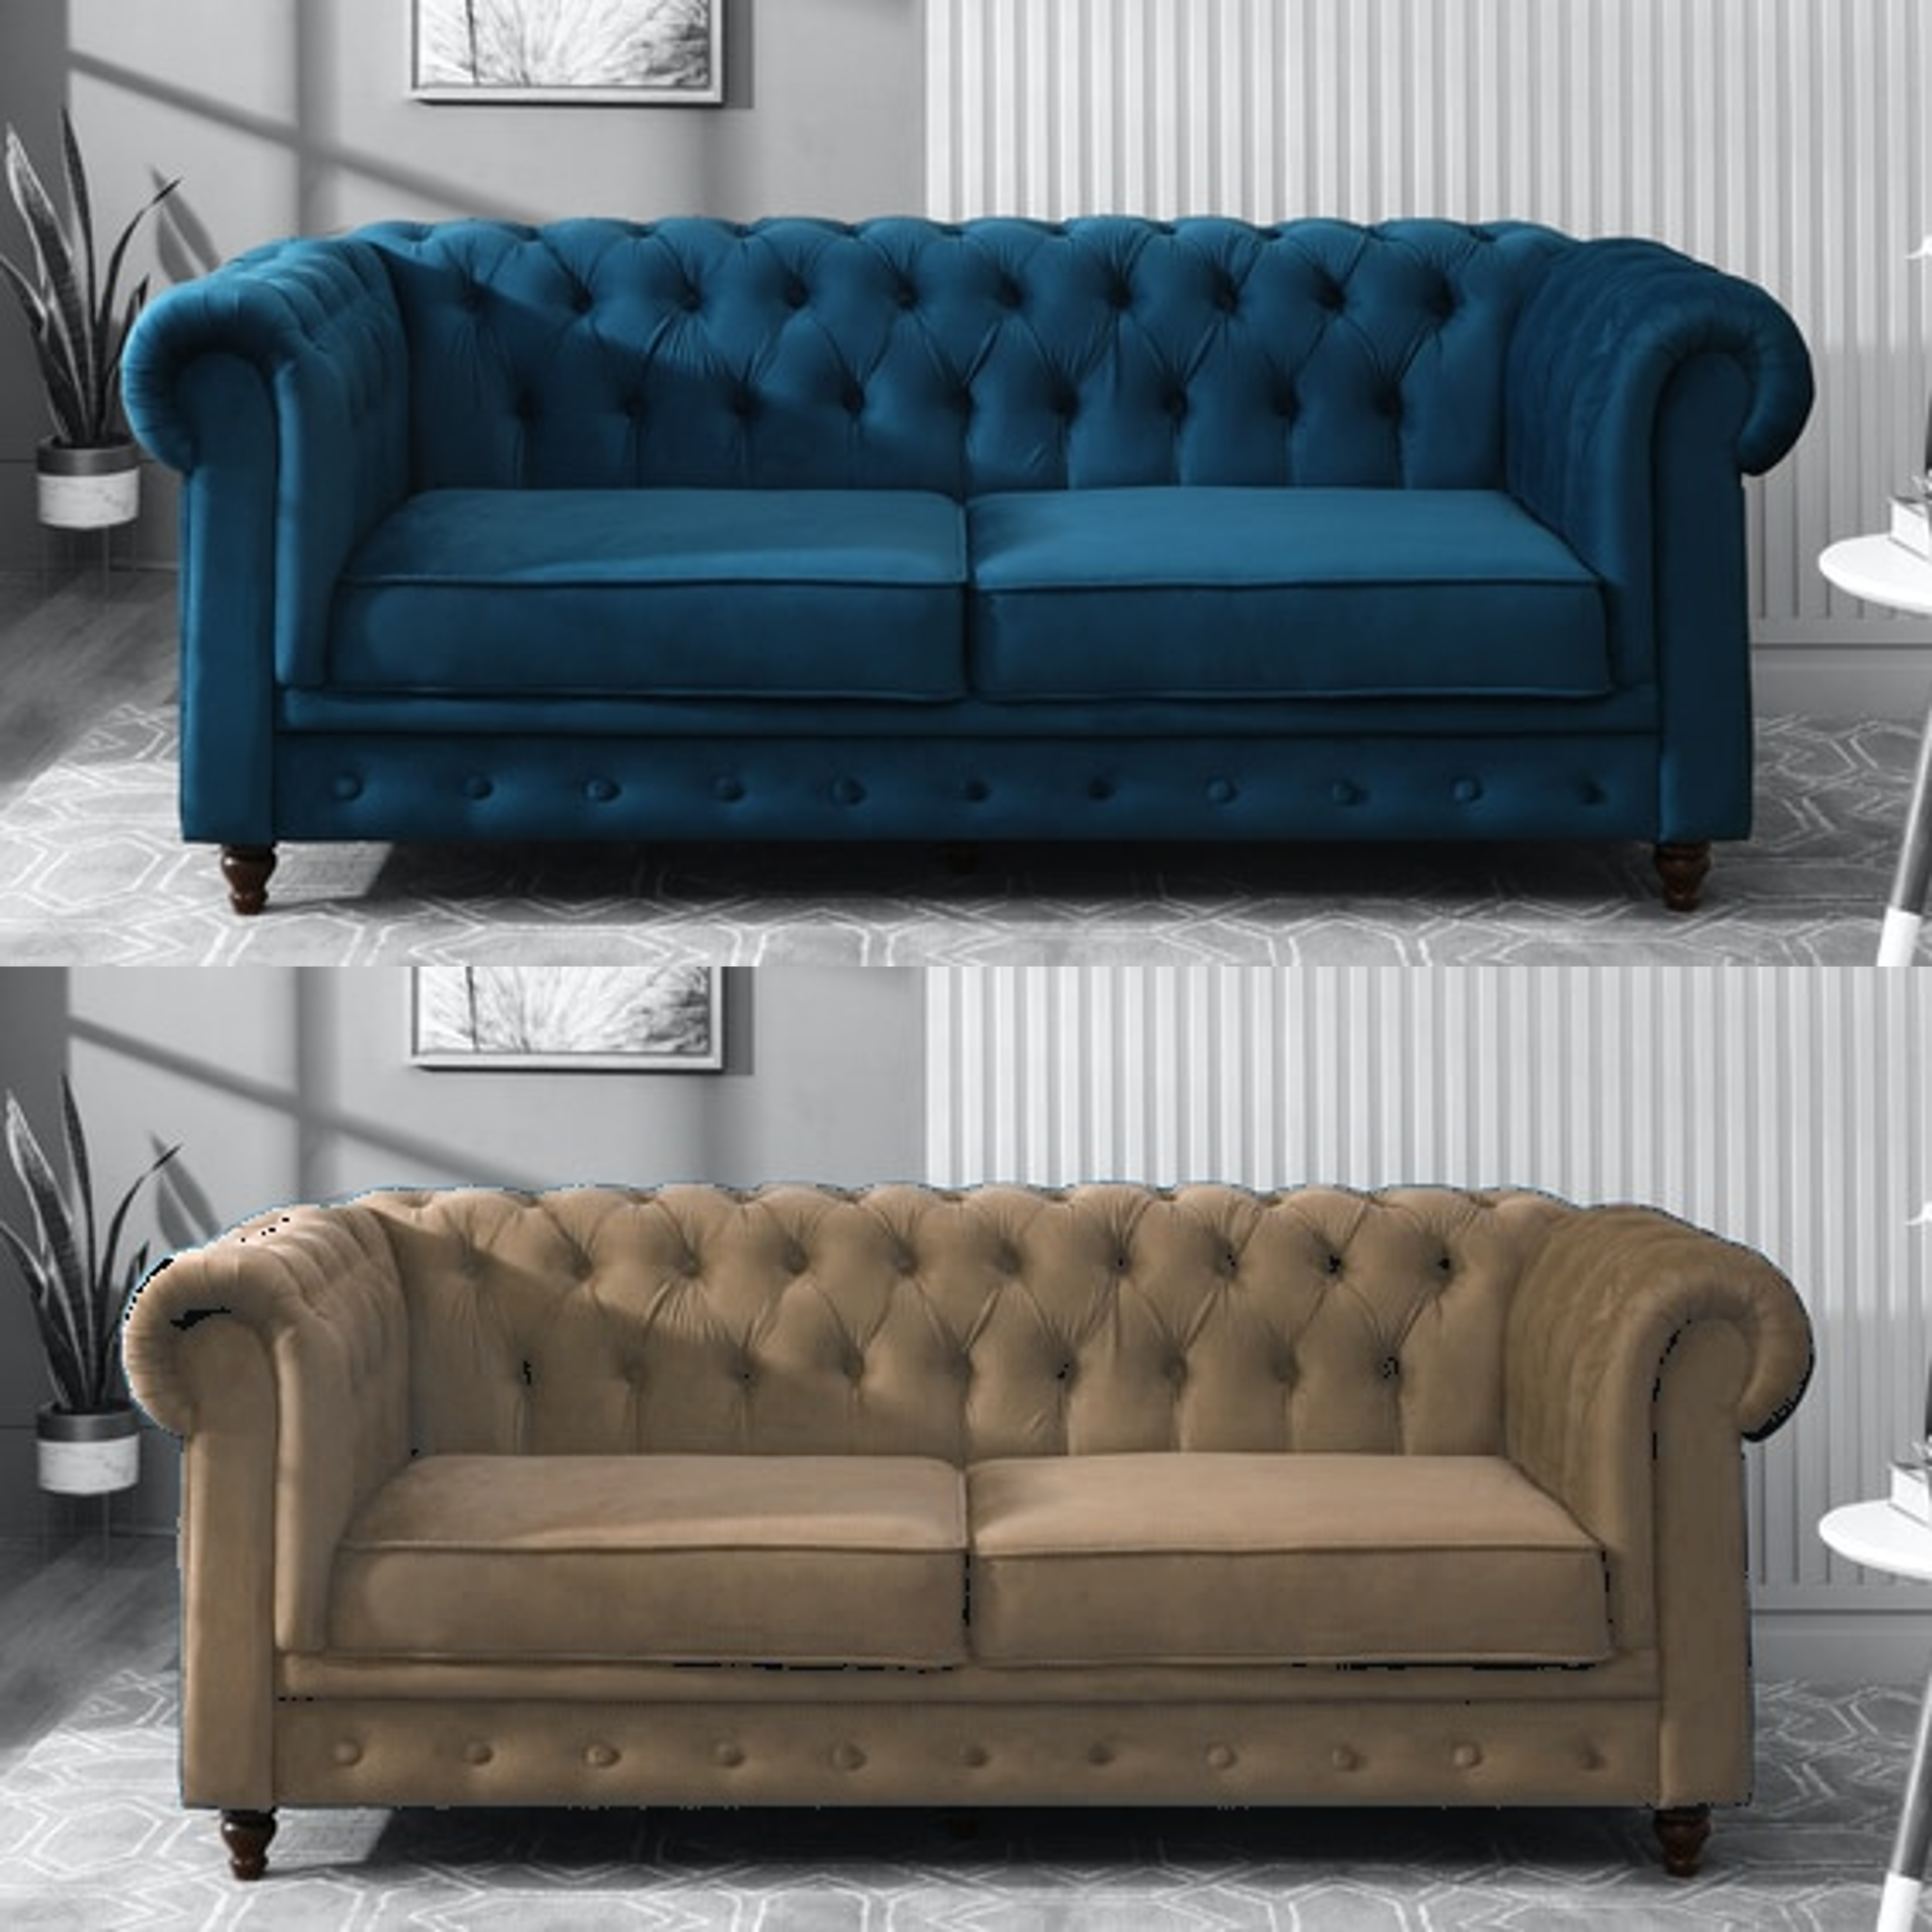
\includegraphics[width=0.5\linewidth]{Figures/boicanh2.png}
\end{figure}
Thay đổi màu của các đối tượng như đồ nội thất, trang phục, trang sức,...
\end{frame}

\begin{frame}{Phát biểu bài toán}
    \begin{table}
        \centering
        \begin{tabular}{ccc}
           \includegraphics[width=0.35\linewidth]{Figures/Picture1.png}  & \includegraphics[width=0.1\linewidth]{Figures/rightarrow.png} &  \includegraphics[width=0.35\linewidth]{Figures/2305_result.png} \\
           Ảnh xám ($I_g$) và điều kiện (c) & & Ảnh được tô màu ($I_{rgb}$)
        \end{tabular}
        \label{tab:my_label}
    \end{table}
    Vì đây là bài toán không đơn trị nên ta có thể mô hình hóa quá trình tô màu như một bài toán sinh mẫu từ một phân phối xác suất có điều kiện:
    \begin{equation*}
             I_{rgb} \sim P(I_{rgb}|I_g,c),
    \end{equation*}
    với c là điều kiện điều khiển quá trình tô màu (nếu có).
\end{frame}

\begin{frame}{Các thách thức của bài toán}

\begin{figure}
    \centering
    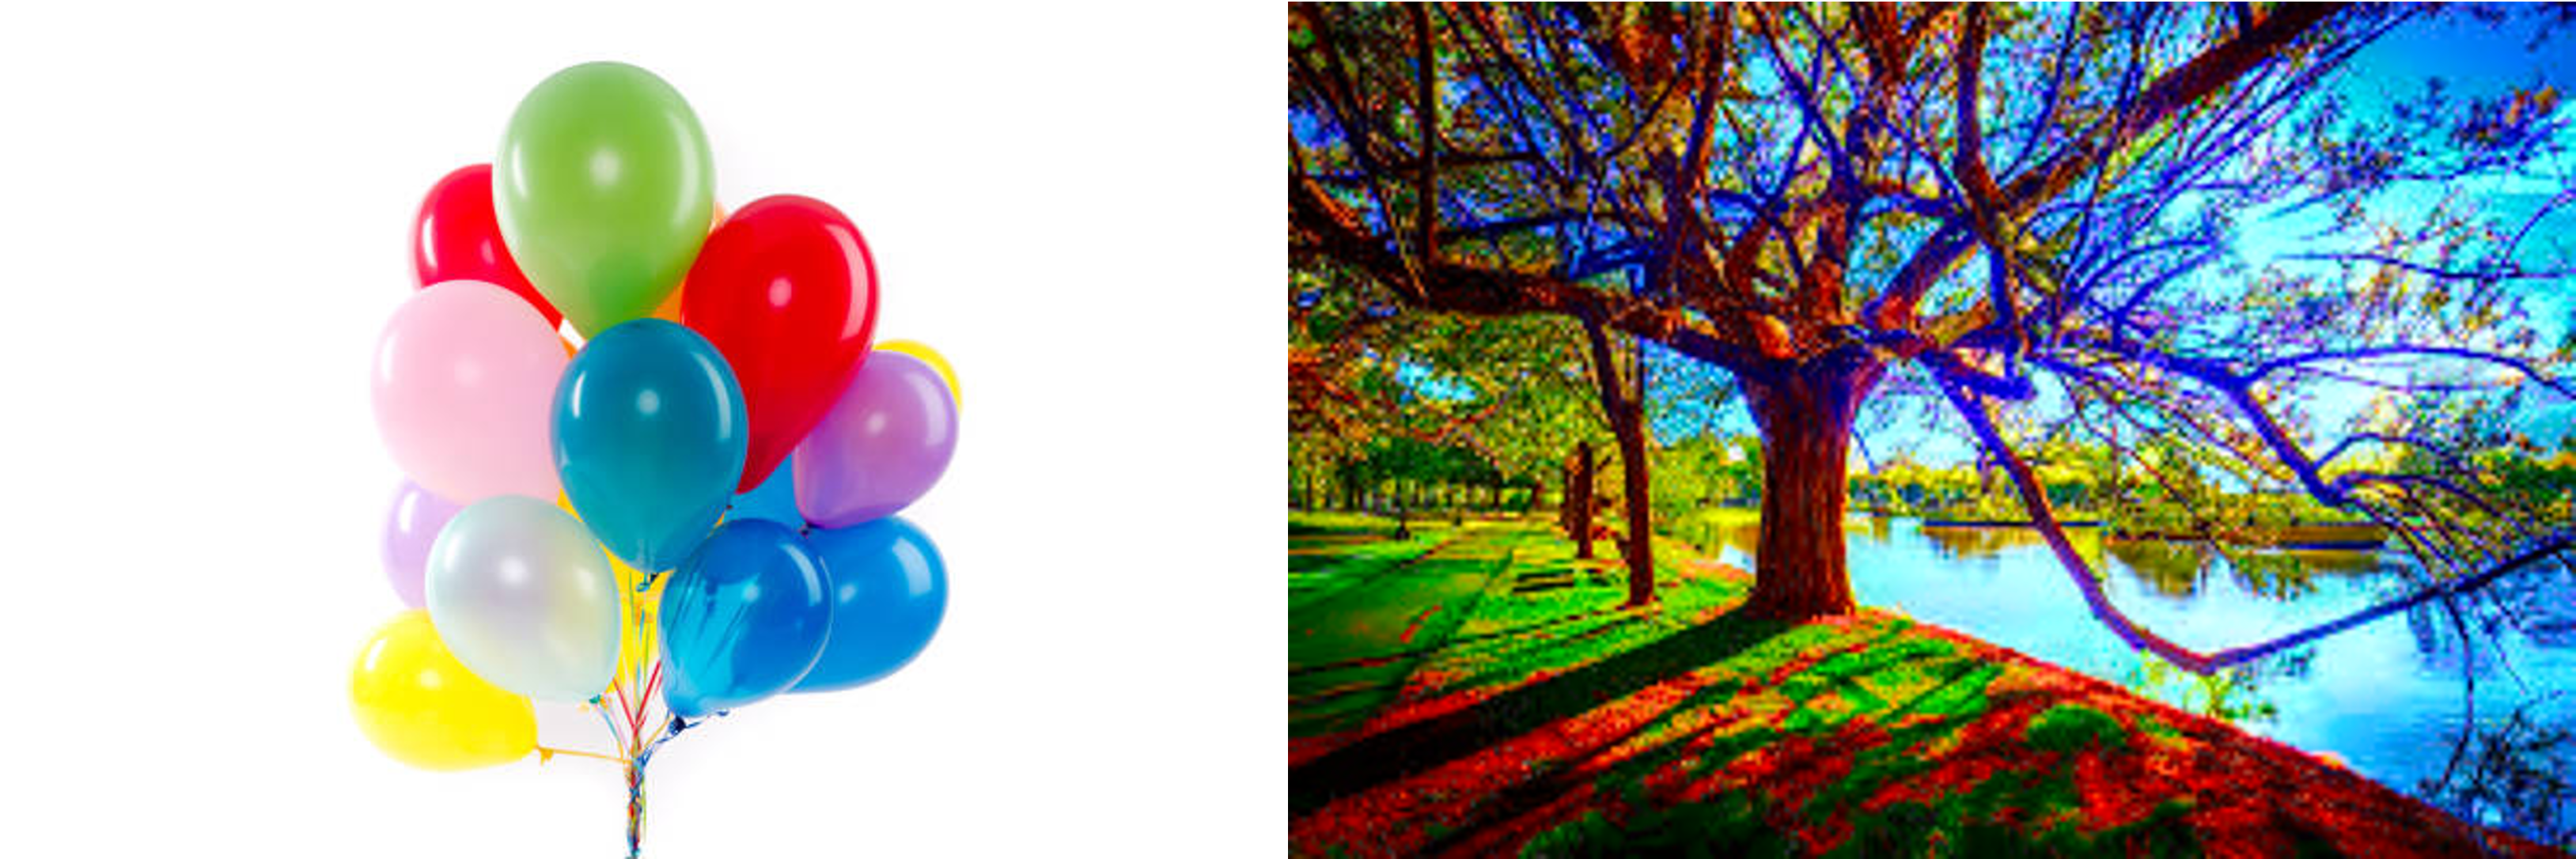
\includegraphics[width=0.8\linewidth]{Figures/hanche.png}
    \label{fig:enter-label}
\end{figure}

\begin{itemize}
    \item Đây là bài toán không đơn trị.

    \item Dễ gặp các lỗi lem màu, tô màu sai.

    \item Yêu cầu tương tác, tốn nhiều thời gian công sức.
\end{itemize}
    
\end{frame}

\begin{frame}{Mục tiêu}
    \begin{itemize}
        \item Xây dựng một mô hình tô màu ảnh độ xám đa phương thức dựa trên mô hình khuếch tán sao cho mô hình ít tiêu tốn tài nguyên trong quá trình huấn luyện và thực thi đồng thời cho ra ảnh màu có chất lượng tốt.
        \item Tìm hiểu sâu hơn về khả năng của các mô hình khuếch tán. Một mô hình đầy mạnh mẽ nhưng chưa được áp dụng quá nhiều vào lĩnh vực tô màu ảnh độ xám.
        \item Tạo ra các mô hình tô màu phục vụ cho các ứng dụng cụ thể.
        \item Tạo ra một giao diện đơn giản có thể giúp người dùng có thể dễ dàng sử dụng các mô hình được xây dựng.
    \end{itemize}
\end{frame}


% ======================================= %
\part{Method}
\tableofcontents[part=2]
\section{Các công trình nghiên cứu liên quan}

% 2 slide:
% - Slide 1: Biểu đồ thể hiện so sánh một số mô hình
% - Slide 2: Chi tiết từng bước bằng chữ, gồm: Tạo sinh mã mẫu từ truy vấn, viết lại mã nguồn trong database, truy vấn

\begin{frame}{Một số mô hình tô màu trước đó}

\begin{table}
    \centering
    \resizebox{\textwidth}{!}{
    \begin{tabular}{p{1.4cm}|p{1.5cm}|p{3cm}|p{3cm}|p{3cm}}
        \toprule
        Mô hình & Kiến trúc & Phương pháp & Ưu điểm & Hạn chế\\
        \midrule
        UniColor & Bộ biến đổi & \small Chuyển các điều kiện đa dạng thành điểm màu gợi ý và tô màu thông qua bộ chuyển đổi & \small Hỗ trợ đa điều kiện; Cho phép chỉnh sửa lại nhiều lần; Kết quả điều khiển khá tốt & \small Phức tạp trong triển khai; Cần xử lý trước mỗi điều kiện riêng biệt \\
        
        BigColor & Mạng đối kháng tạo sinh & \small Học cách tạo sinh màu bằng GAN dựa trên cấu trúc không gian sẵn có của ảnh xám đầu vào & \small Có thể sinh ra nhiều kết quả tô màu khác nhau; Hỗ trợ độ phân giải ảnh kết quả linh hoạt & \small Kém hiệu quả với các ảnh phức tạp hoặc chi tiết nhỏ; Không hỗ trợ tương tác trực tiếp \\
        
        Palette & Khuếch tán & \small Học một mô hình khuếch tán được huấn luyện bằng điều kiện ảnh độ xám & \small Tổng quát, hiệu năng cao; Kết quả vượt GAN trong nhiều thí nghiệm & \small Chậm do sinh mẫu qua nhiều bước; Không hỗ trợ điều kiện; Tốn nhiều tài nguyên \\
        \bottomrule
    \end{tabular}
    }
    \label{tab:my_label}
\end{table}

\end{frame}


\begin{frame}{Ý tưởng từ mô hình ControlColor}
    \begin{figure}
        \centering
        \includegraphics[width=0.8\linewidth]{Figures/ControlColor.png}
        \label{fig:enter-label}
    \end{figure}
    \textbf{Khuyết điểm:} Mô hình quá phức tạp cũng như yêu cầu quá nhiều tài nguyên cho quá trình huấn luyện và thực thi để đạt được kết quả tốt.
\end{frame}





%----------------------------------------
\part{Similarity metrics}
\tableofcontents[part=3]
\section{Mô hình đề xuất}

% 2 slides:
% - Slide 1: Giới thiệu về ControlNet và LDM
% - Slide 2: Giới thiệu về mô hình huấn luyện và thực thi

\begin{frame}{Kiến trúc ControlNet}

    \begin{figure}
        \centering
        \includegraphics[width=0.6\linewidth]{Figures/controlnet_arch.png}
        % \caption{Kiến trúc mô hình ControlNet}
    \end{figure}

Kiến trúc ControlNet giúp thêm điều kiện điều khiển không gian vào các mô hình tạo sinh ảnh từ văn bản được huấn luyện sẵn.

\end{frame}


\begin{frame}{Mô hình khuếch tán trong không gian tiềm ẩn}

\begin{figure}
    \centering
    \includegraphics[width=0.9\linewidth]{Figures/LDM_arch.png}
     % \caption{Kiến trúc mô hình khuếch tán trong không gian tiềm ẩn}
\end{figure}

Sử dụng mô hình tiền huấn luyện Stable Diffusion được huấn luyện trên 2 tỉ cặp ảnh và văn bản của tập dữ liệu LAION.

\end{frame}

\begin{frame}{Mô hình đề xuất}

    \begin{figure}
        \centering
        \includegraphics[width=0.9\linewidth]{Figures/main_model.png}
        % \caption{Kiến trúc mô hình đề xuất}
    \end{figure}


   
\end{frame}
%----------------------------------------
\part{Experiment and Evaluation}
\tableofcontents[part=4]
\section{Thực nghiệm}

% 4 slides:
% - Side 1: Giới thiệu các tập data đc sử dụng
% - Slide 2: So sánh ReCo với các phương pháp khác (GAR, BM25, UniXcoder, CodeT5+)
% - Slide 3: Kết quả đánh giá trên các tập dữ liệu
% - Slide 4: So sánh CSSim với các độ đo khác (BLEU, ROUGE-L, CodeBLEU)

\subsection*{Huấn luyện}

% - tập dữ liệu ImageNet100k dùng để huấn luyện mô hình tổng quát, với mong muốn tô màu trên nhiều miền ảnh nhất có thể.
% - ba tập dữ liệu còn lại dùng để huấn luyện các mô hình tô màu trên miền ảnh chuyên biệt, bao gồm thời trang, nội thất, và khuôn mặt

\begin{frame}{Tập dữ liệu}
\begin{itemize}
    \item \textbf{ImageNet100k}: bao gồm 100K ảnh được chọn ngẫu nhiên từ tập dữ liệu huấn luyện ImageNet.
    \item \textbf{Fashion Product Images}: bao gồm khoảng 44K ảnh, mỗi ảnh chứa một loại phụ kiện thời trang chính, có thể được chụp với người mẫu hoặc chụp trên nền trắng.
    \item \textbf{Furniture Image}: bao gồm 15K ảnh của 5 loại nội thất khác nhau (tủ quần áo, ghế, tủ lạnh, bàn, tivi).
    \item \textbf{VN-celeb}: bao gồm khoảng 23K khuôn mặt của 1.020 người nổi tiếng ở Việt Nam có thế tìm thấy trên mạng, cụ thể là Wikipedia Việt Nam.
\end{itemize}    
\end{frame}
% các tập dữ liệu sẽ được tiền xử lý qua 3 bước:
% - lọc các ảnh tương đối xám, chỉ giữa lại các ảnh  màu sắc ổn định để huấn luyện
% - điều chỉnh về cùng 1 độ phân giải
% - tạo sinh câu mô tả bằng mô hình BLIP để làm điều kiện cho quá trình huấn luyệnluyện

\begin{frame}{Tiền xử lý dữ liệu}
    \begin{enumerate}
        \item Lọc ảnh độ xám: loại bỏ các ảnh có màu sắc tương đối xám, chỉ giữ lại các ảnh có màu sắc ổn định cho việc huấn luyện.
        \[
          E(Var(C_i,C_j)) = \frac{1}{3}\sum_{(i,j) \in \{(R,G),(G,B),(B,R)\}} Var(C_i - C_j) < t
        \]
        \item Thay đổi độ phân giải: về cùng kích thước $512 \times 512$.
        \item Tạo sinh câu mô tả: sử dụng mô hình BLIP sinh câu mô tả để làm điều kiện trong quá trình huấn luyện.
    \end{enumerate}
\vspace{0.3cm}
Dữ liệu cho việc huấn luyện được tổ chức theo bộ ba tương ứng là: \textbf{ảnh xám, ảnh màu, câu mô tả}.
\vspace{-3mm}
\begin{table}[ht]
    \centering
    \resizebox{\textwidth}{!}{
    \begin{tabular}{c|cccc}
        \toprule
        Tập dữ liệu & ImageNet100k & Fashion Product Images & Furniture Image & VN-celeb \\
        \midrule
        Số lượng ảnh & 97,590 & 38,284 & 13,525 & 22,284 \\
        \bottomrule
    \end{tabular}
}
    % \caption{Thống kê số lượng ảnh theo từng tập huấn luyện sau khi tiền xử lý.}
    % \label{tab:train-dataset}
\end{table}

\end{frame}

% \begin{frame}{Triển khai}
%     \begin{itemize}
%         \item Sử dụng mô hình tiền huấn luyện tạo sinh ảnh Stable Duffusion V1.5.
%         \item Ảnh đầu vào $512 \times 512$ được nén vào không gian tiềm ẩn với kích thước $64 \times 64$ và được giải mã bằng bộ mã hóa tự động.
%         \item Sử dụng bộ mã hóa văn bản CLIP ViT-L14 để mã hóa câu mô tả thành vec-tơ có chiều dài 768.
%         \item Dùng kiến thức U-Net kết hợp với cơ chế chú ý chéo (8 đầu) để kết hợp thông tin văn bản và thời gian.
%         \item Sử dụng hàm tối ưu Adam với tham số $\beta_1 = 0.9$ và $\beta_2 = 0.999$, tốc độ học là $10^{-5}$.
%         \item Huấn luyện mô hình chính trên tập ImageNet100k với 10,674 bước trong 2 ngày, với kích thước lô là 8.
%         \item Các mô hình trong nghiên cứu đều được huấn luyện với RAM 64GB và 1 GPU A100 với 40GB VRAM từ máy chủ do Khoa cung cấp.
%     \end{itemize}
% \end{frame}

% \begin{frame}{Kết quả quá trình huấn luyện}
%     Có nên viết hay không ?
% \end{frame}

\subsection*{Đánh giá}
% - Độ đo FID và Colorfulness được dùng để đánh giá tất cả phương thức tô màu của mô hình
% - Điểm số CLIP được dùng riêng cho đánh giá phương thức tô màu dựa trên câu mô tả

\begin{frame}{Độ đo}
Có ba độ đo phổ biến trong các nghiên cứu tô màu ảnh độ xám, gồm:
\begin{itemize}
    \item \textbf{Độ đo Fréchet Inception Distance (FID)} - kiểm tra độ chân thật của ảnh được tạo ra so với ảnh gốc. Ảnh sinh ra càng giống ảnh gốc thì FID càng thấp.
    \item \textbf{Độ đo Colorfulness} - đánh giá độ sặc sỡ của ảnh được tô màu. Ảnh càng sặc sỡ thì Colorfulness càng cao.
    \item \textbf{Điểm số CLIP} - đánh giá độ tương đồng giữa ảnh kết quả với câu mô tả trong không gian tiềm ẩn của CLIP, được dùng cho phương thức tô màu bán tự động.
    
    % \[
    %     \text{CLIP score} = \dfrac{\mathrm{I} \cdot \mathrm{T}}{||\mathrm{I}||\cdot ||\mathrm{T}||}
    % \]
    % trong đó, $\mathrm{I} = \epsilon_i(i)$ và $\mathrm{T} = \epsilon_t(t)$, lần lượt là vec-tơ mã hóa của ảnh và văn bản của hai bộ mã hóa tương ứng.
\end{itemize}
\end{frame}


\begin{frame}{Chiến lược đánh giá}
    \begin{enumerate}
        \item So sánh chất lượng với các mô hình SOTA
        \item So sánh Mô hình tổng quát với các mô hình chuyện biệt
        % \item Đánh giá sự phụ thuộc của chất lượng ảnh vào các tham số của mô hình
    \end{enumerate}
\end{frame}

% \begin{frame}{Tô màu tự động - Tập dữ liệu}
%     \begin{itemize}
%         \item val5k: gồm 5K ảnh đầu tiên trong tập đánh giá của ImageNet.
%         \item ctest: gồm 10K ảnh được lấy ngẫu nhiên của tập đánh giá của ImageNet.
%         \item COCO-Stuff: gồm 5K ảnh của tập đánh giá của bộ dữ liệu COCO-Stuff.
%     \end{itemize}
% \end{frame}

\begin{frame}{Tô màu tự động - Kết quả}
% So sánh với các mô hình  thuộc 3 nhóm kiến trúc: mạng đối kháng, bộ biến đổi và khuếch tán (GAN, Transformer và Diffusion)
% Với độ đo Colorfulness, nhóm đạt thứ hạng 2, chỉ thua mô hình Control Color
% Với độ đo FID, tuy không tốt hơn mô hình DDColor, nhưng nhóm đạt độ hiểu quả ở mức độ trung bình, vẫn tốt hơn phần lớn mô hình còn lại.
% Điểm chú ý là mô hình đề xuất vẫn đạt độ hiệu quả cao, trong khi chi phí huấn luyện với ít dữ liệu và ít bước hơn nhiều so với các mô hình còn lại.
    \begin{table}[ht]
            \centering
            \resizebox{\textwidth}{!}{
                \begin{tabular}{c |c c | c c | c c}
                    \toprule
                    Tập dữ liệu & \multicolumn{2}{c|}{ImageNet (val5k)} & \multicolumn{2}{c|}{ImageNet (ctest)} & \multicolumn{2}{c}{COCO-Stuff} \\
                    \cmidrule(lr){2-3} \cmidrule(lr){4-5} \cmidrule(lr){6-7}
                    Độ đo & FID$\downarrow$ & Colorfulness$\uparrow$ & FID$\downarrow$ & Colorfulness$\uparrow$ & FID$\downarrow$ & Colorfulness$\uparrow$ \\
                    \midrule
                    CIC & 22.0860 & 37.0313 & 12.7651 & 37.5761 & 33.3418 & 37.6487 \\
                    UGColor & 15.1777 & 27.0966 & 6.5466 & 27.8122 & 21.4010 & 28.4487 \\
                    DeOldify & 10.5191 & 26.4827 & 4.2143 & 23.1538 & 13.4318 & 28.3779 \\
                    ChromaGAN & 16.4390  & 25.5862 & 9.3487 & 29.0895 & 26.4624 & 29.1411 \\
                    InstColor & 12.9455 & 27.5710 & 6.7803 & 28.1923 & 12.6844 & 29.2302 \\
                    ToVivid & \underline{5.8019}  & 37.3376 &\underline{2.6775} & 37.8425 & 8.5452 & 38.8155 \\
                    BigColor & 7.7677  & 42.5364 & 2.8583 & 44.4135 & 10.0362 & 43.4104 \\
                    \midrule
                    DISCO & 10.2895 & 40.9533 & 5.7196 & 37.4613 & 13.3850 & 39.1969 \\
                    DDColor & \textbf{5.5726} & 42.8370 & \textbf{2.6294} & 42.9575 & \textbf{7.2718} & 42.2919 \\
                    ColorFormer & 6.3831  & 40.5631 & 2.9816 & 41.2833 & 8.5623 & 41.0248 \\
                    UniColor & 9.6292  & 36.3415 & 4.9140 & 37.1726 & \underline{8.0509} & 36.7442 \\
                    \midrule
                    Control Color & 8.8749 & \textbf{47.1680} & 4.2915 & \textbf{44.9256} & 10.2651 & \textbf{47.0501}\\
                    \midrule
                    \textbf{ColorFill-LDM-CNet} & 10.4125 & \underline{44.2871} & 6.8341 & \underline{44.7854} & 10.4632         & \underline{45.2589} \\
                    \bottomrule
                \end{tabular}
            }
            % \caption{So sánh định lượng khả năng tô màu tự động của các mô hình.}
            % trên các tập dữ liệu ImageNet (val5k), ImageNet (ctest) và COCO-Stuff. Số liệu được \textbf{in đậm} thể hiện kết quả tốt nhất, số liệu tốt thứ hai được thể hiện bằng cách \underline{gạch chân}.}
            \label{tab:uncond-metrics}
        \end{table}
\end{frame}

\begin{frame}{Tô màu tự động - Kết quả (tt)}
% - Đây là một số mẫu ảnh được tô màu bởi mô hình đề xuất và một số mô hình khác.
% - Một số ảnh như chim cánh cụt (ở mô hình Unicolor hoặc BigColor) rất sặc sỡ nhưng không đúng với màu trong tự nhiên
% - Ở các mô hình ToViVid và DDColor, có độ đo FID cao nhất như theo bảng số liệu trước. Vì chúng hiệu quả ở phía cạnh tô màu chân thật, nên màu sắc của ảnh được tô không phong phú, bị đều màu và có phần hơi nhạt.
% - Trong khi đó, ảnh được tạo ra từ mô hình của nhóm vừa sặc sỡ, vừa rất chân thật, màu của các đối tượng được tô đúng với thực tế.

   \begin{figure}[htp]
        	\centering
        	\begin{tabular}{@{}c@{}c@{\hspace{0.1em}}c@{\hspace{0.1em}}c@{\hspace{0.1em}}c@{\hspace{0.1em}}c@{\hspace{0.1em}}c@{\hspace{0.1em}}c@{}}
        		\includegraphics[width=0.05\linewidth]{Figures/header/anh_goc.png} & 
        		\includegraphics[width=0.12\linewidth]{Figures/gt/ILSVRC2012_val_00004780.JPEG} & 
        		\includegraphics[width=0.12\linewidth]{Figures/gt/ILSVRC2012_val_00004581.JPEG} & 
        		\includegraphics[width=0.12\linewidth]{Figures/gt/ILSVRC2012_val_00003989.JPEG} & 
        		\includegraphics[width=0.12\linewidth]{Figures/gt/ILSVRC2012_val_00001859.JPEG} & 
        		\includegraphics[width=0.12\linewidth]{Figures/gt/ILSVRC2012_val_00003625.JPEG} & 
        		\includegraphics[width=0.12\linewidth]{Figures/gt/ILSVRC2012_val_00002305.JPEG} & 
        		\includegraphics[width=0.12\linewidth]{Figures/gt/ILSVRC2012_val_00002437.JPEG} \\ [-3pt]   
        		
        		% \includegraphics[width=0.05\linewidth]{Figures/header/anh_dau_vao.png} &
        		% \includegraphics[width=0.12\linewidth]{Figures/inputs/ILSVRC2012_val_00004780.JPEG} & 
        		% \includegraphics[width=0.12\linewidth]{Figures/inputs/ILSVRC2012_val_00004581.JPEG} & 
        		% \includegraphics[width=0.12\linewidth]{Figures/inputs/ILSVRC2012_val_00003989.JPEG} & 
        		% \includegraphics[width=0.12\linewidth]{Figures/inputs/ILSVRC2012_val_00001859.JPEG} & 
        		% \includegraphics[width=0.12\linewidth]{Figures/inputs/ILSVRC2012_val_00003625.JPEG} & 
        		% \includegraphics[width=0.12\linewidth]{Figures/inputs/ILSVRC2012_val_00002305.JPEG} & 
        		% \includegraphics[width=0.12\linewidth]{Figures/inputs/ILSVRC2012_val_00002437.JPEG} \\ [-3pt]
        		\includegraphics[width=0.05\linewidth]{Figures/header/unicolor.png} &
        		\includegraphics[width=0.12\linewidth]{Figures/uni_rs/ILSVRC2012_val_00004780.JPEG} & 
        		\includegraphics[width=0.12\linewidth]{Figures/uni_rs/ILSVRC2012_val_00004581.JPEG} & 
        		\includegraphics[width=0.12\linewidth]{Figures/uni_rs/ILSVRC2012_val_00003989.JPEG} & 
        		\includegraphics[width=0.12\linewidth]{Figures/uni_rs/ILSVRC2012_val_00001859.JPEG} & 
        		\includegraphics[width=0.12\linewidth]{Figures/uni_rs/ILSVRC2012_val_00003625.JPEG} & 
        		\includegraphics[width=0.12\linewidth]{Figures/uni_rs/ILSVRC2012_val_00002305.JPEG} & 
        		\includegraphics[width=0.12\linewidth]{Figures/uni_rs/ILSVRC2012_val_00002437.JPEG} \\ [-3pt]
        		\includegraphics[width=0.05\linewidth]{Figures/header/bigcolor.png} &
        		\includegraphics[width=0.12\linewidth]{Figures/big_color_rs/ILSVRC2012_val_00004780_c150.jpg} & \includegraphics[width=0.12\linewidth]{Figures/big_color_rs/ILSVRC2012_val_00004581_c911.jpg} & \includegraphics[width=0.12\linewidth]{Figures/big_color_rs/ILSVRC2012_val_00003989_c872.jpg} & \includegraphics[width=0.12\linewidth]{Figures/big_color_rs/ILSVRC2012_val_00001859_c718.jpg} & \includegraphics[width=0.12\linewidth]{Figures/big_color_rs/ILSVRC2012_val_00003625_c989.jpg} & \includegraphics[width=0.12\linewidth]{Figures/big_color_rs/ILSVRC2012_val_00002305_c310.jpg} & \includegraphics[width=0.12\linewidth]{Figures/big_color_rs/ILSVRC2012_val_00002437_c883.jpg} \\ [-3pt]
        		\includegraphics[width=0.05\linewidth]{Figures/header/tovid.png} &
        		\includegraphics[width=0.12\linewidth]{Figures/vivid_rs/ILSVRC2012_val_00004780.png} & 
        		\includegraphics[width=0.12\linewidth]{Figures/vivid_rs/ILSVRC2012_val_00004581.png} & 
        		\includegraphics[width=0.12\linewidth]{Figures/vivid_rs/ILSVRC2012_val_00003989.png} & 
        		\includegraphics[width=0.12\linewidth]{Figures/vivid_rs/ILSVRC2012_val_00001859.png} & 
        		\includegraphics[width=0.12\linewidth]{Figures/vivid_rs/ILSVRC2012_val_00003625.png} & 
        		\includegraphics[width=0.12\linewidth]{Figures/vivid_rs/ILSVRC2012_val_00002305.png} & 
        		\includegraphics[width=0.12\linewidth]{Figures/vivid_rs/ILSVRC2012_val_00002437.png} \\ [-3pt]
        		\includegraphics[width=0.05\linewidth]{Figures/header/ddcolor.png} &
        		\includegraphics[width=0.12\linewidth]{Figures/ddcolor_rs/ILSVRC2012_val_00004780.JPEG} & 
        		\includegraphics[width=0.12\linewidth]{Figures/ddcolor_rs/ILSVRC2012_val_00004581.JPEG} & 
        		\includegraphics[width=0.12\linewidth]{Figures/ddcolor_rs/ILSVRC2012_val_00003989.JPEG} & 
        		\includegraphics[width=0.12\linewidth]{Figures/ddcolor_rs/ILSVRC2012_val_00001859.JPEG} & 
        		\includegraphics[width=0.12\linewidth]{Figures/ddcolor_rs/ILSVRC2012_val_00003625.JPEG} & 
        		\includegraphics[width=0.12\linewidth]{Figures/ddcolor_rs/ILSVRC2012_val_00002305.JPEG} & 
        		\includegraphics[width=0.12\linewidth]{Figures/ddcolor_rs/ILSVRC2012_val_00002437.JPEG} \\ [-3pt]
        		\includegraphics[width=0.05\linewidth]{Figures/header/colorfill.png} &
        		\includegraphics[width=0.12\linewidth]{Figures/main_rs/ILSVRC2012_val_00004780.png} & 
        		\includegraphics[width=0.12\linewidth]{Figures/main_rs/ILSVRC2012_val_00004581.png} & 
        		\includegraphics[width=0.12\linewidth]{Figures/main_rs/ILSVRC2012_val_00003989.png} & 
        		\includegraphics[width=0.12\linewidth]{Figures/main_rs/ILSVRC2012_val_00001859.png} & 
        		\includegraphics[width=0.12\linewidth]{Figures/main_rs/ILSVRC2012_val_00003625.png} & 
        		\includegraphics[width=0.12\linewidth]{Figures/main_rs/ILSVRC2012_val_00002305.png} & 
        		\includegraphics[width=0.12\linewidth]{Figures/main_rs/ILSVRC2012_val_00002437.png} \\ [-3pt]      
        	\end{tabular}
        	% \caption{Kết quả so sánh trực quan mô hình của nhóm (chúng tôi) với một số mô hình tô màu trước đó trên phương thức tô màu tự động. Ảnh đầu vào được lấy từ tập thử nghiệm ImageNet (val5k).}
        	\label{fig:sample}
        
        \end{figure}
\end{frame}

\begin{frame}{Tô màu tự động - Kết quả (tt)}
% Như đã trình bày, mô hình của nhóm kém hơn mô hình Control Color ở độ đo Colorfulness.
% Tuy nhiên, một số tình huống, ảnh do Control Color tạo ra đúng là sặc sỡ hơn, nhưng nhìn bằng mắt có thể thấy các ảnh đó không tốt bằng ảnh do mô hình đề xuất tạo ra.
% ở bức ảnh có con chó, thì màu xanh của cỏ bị tràn sang 2 vùng bê tông xung quanh.
% ở bức ảnh con tàu, thì nước biển lại được tô màu vàng, không đúng với thực tế.
   \begin{figure}[htp]
        	\centering
        	\begin{tabular}{@{}c@{}c@{\hspace{0.1em}}c@{\hspace{0.1em}}c@{\hspace{0.1em}}c@{\hspace{0.1em}}c@{\hspace{0.1em}}c@{\hspace{0.1em}}c@{}}
        		\includegraphics[width=0.1\linewidth]{Figures/header/anh_goc.png} &
        		\includegraphics[width=0.13\linewidth]{Figures/gt/ILSVRC2012_val_00001400.JPEG} &
        		\includegraphics[width=0.16\linewidth]{Figures/gt/ILSVRC2012_val_00002503.JPEG} &
        		\includegraphics[width=0.26\linewidth]{Figures/gt/ILSVRC2012_val_00002748.JPEG} &
        		\includegraphics[width=0.26\linewidth]{Figures/gt/ILSVRC2012_val_00004780.JPEG} \\ [-3pt]

        		% \includegraphics[width=0.05\linewidth]{Figures/header/anh_dau_vao.png} &
        		% \includegraphics[width=0.13\linewidth]{Figures/inputs/ILSVRC2012_val_00004780.JPEG} &
        		% \includegraphics[width=0.13\linewidth]{Figures/inputs/ILSVRC2012_val_00004581.JPEG} &
        		% \includegraphics[width=0.13\linewidth]{Figures/inputs/ILSVRC2012_val_00003989.JPEG} &
        		% \includegraphics[width=0.13\linewidth]{Figures/inputs/ILSVRC2012_val_00001859.JPEG} &
        		% \includegraphics[width=0.13\linewidth]{Figures/inputs/ILSVRC2012_val_00003625.JPEG} &
        		% \includegraphics[width=0.13\linewidth]{Figures/inputs/ILSVRC2012_val_00002305.JPEG} &
        		% \includegraphics[width=0.13\linewidth]{Figures/inputs/ILSVRC2012_val_00002437.JPEG} \\ [-3pt]
        		\includegraphics[width=0.05\linewidth]{Figures/header/controlcolor.png} &
        		\includegraphics[width=0.13\linewidth]{Figures/ctrlcolor/16181/ILSVRC2012_val_00001400.png} &
        		\includegraphics[width=0.16\linewidth]{Figures/ctrlcolor/16181/ILSVRC2012_val_00002503.png} &
        		\includegraphics[width=0.26\linewidth]{Figures/ctrlcolor/16181/ILSVRC2012_val_00002748.png} &
        		\includegraphics[width=0.26\linewidth]{Figures/ctrlcolor/16181/ILSVRC2012_val_00004780.png} \\ [-3pt]

				\includegraphics[width=0.05\linewidth]{Figures/header/colorfill-2.png} &
        		\includegraphics[width=0.13\linewidth]{Figures/main_rs/ILSVRC2012_val_00001400.png} &
        		\includegraphics[width=0.16\linewidth]{Figures/main_rs/ILSVRC2012_val_00002503.png} &
        		\includegraphics[width=0.26\linewidth]{Figures/main_rs/ILSVRC2012_val_00002748.png} &
        		\includegraphics[width=0.26\linewidth]{Figures/main_rs/ILSVRC2012_val_00004780.png} & \\ [-3pt]

				% \includegraphics[width=0.03\linewidth]{Figures/header/colorfill-2.png} &
        		% \includegraphics[width=0.13\linewidth]{Figures/main_rs/ILSVRC2012_val_00004780.png} &
        		% \includegraphics[width=0.13\linewidth]{Figures/main_rs/ILSVRC2012_val_00004581.png} &
        		% \includegraphics[width=0.13\linewidth]{Figures/main_rs/ILSVRC2012_val_00003989.png} &
        		% \includegraphics[width=0.13\linewidth]{Figures/main_rs/ILSVRC2012_val_00001859.png} &
        		% \includegraphics[width=0.13\linewidth]{Figures/main_rs/ILSVRC2012_val_00003625.png} &
        		% \includegraphics[width=0.13\linewidth]{Figures/main_rs/ILSVRC2012_val_00002305.png} &
        		% \includegraphics[width=0.13\linewidth]{Figures/main_rs/ILSVRC2012_val_00002437.png} \\ [-3pt]
        	\end{tabular}
        	\caption{Kết quả so sánh trực quan mô hình của nhóm (ColorFill-LDM-CNet) với mô hình Control Color trên phương thức tô màu tự động. Ảnh đầu vào được lấy từ tập thử nghiệm ImageNet (val5k).}
        	\label{fig:sample}

        \end{figure}
\end{frame}
\begin{frame}{Tô màu tự động - Kết quả (tt)}
% Tuy nhiên, mô hình của nhóm vẫn có một số hạn chế như:
% Mô hình của nhóm kém khi cố gắng tô màu các đối tượng ở phần background của ảnh (như hình gấu bông hoặc người phụ nữ) hoặc ở ảnh người đàn ông thổi kèn, tuy ảnh sau khi được tô có thể chấp nhận được nhưng màu sắc không đa dạng bằng của Control Color.
    \begin{figure}[htp]
        	\centering
        	\begin{tabular}{@{}c@{}c@{\hspace{0.1em}}c@{\hspace{0.1em}}c@{\hspace{0.1em}}c@{\hspace{0.1em}}c@{\hspace{0.1em}}c@{\hspace{0.1em}}c@{}}
        		\includegraphics[width=0.1\linewidth]{Figures/header/anh_goc.png} &
        		\includegraphics[width=0.13\linewidth]{Figures/gt/ILSVRC2012_val_00003759.JPEG} &
				\includegraphics[width=0.23\linewidth]{Figures/gt/ILSVRC2012_val_00004581.JPEG} &
        		\includegraphics[width=0.26\linewidth]{Figures/gt/ILSVRC2012_val_00001085.JPEG}\\ [-3pt]

        		\includegraphics[width=0.05\linewidth]{Figures/header/controlcolor.png} &
        		\includegraphics[width=0.13\linewidth]{Figures/ctrlcolor/16181/ILSVRC2012_val_00003759.png} &
				\includegraphics[width=0.23\linewidth]{Figures/ctrlcolor/16181/ILSVRC2012_val_00004581.png} &
        		\includegraphics[width=0.26\linewidth]{Figures/ctrlcolor/16181/ILSVRC2012_val_00001085.png}\\ [-3pt]

				\includegraphics[width=0.05\linewidth]{Figures/header/colorfill-2.png} &
        		\includegraphics[width=0.13\linewidth]{Figures/main_rs/ILSVRC2012_val_00003759.png} &
				\includegraphics[width=0.23\linewidth]{Figures/main_rs/ILSVRC2012_val_00004581.png} &
        		\includegraphics[width=0.26\linewidth]{Figures/main_rs/ILSVRC2012_val_00001085.png}\\ [-3pt]

        	\end{tabular}
        	% \caption{Kết quả so sánh trực quan mô hình của nhóm (ColorFill-LDM-CNet) với mô hình Control Color trên phương thức tô màu tự động. Ảnh đầu vào được lấy từ tập thử nghiệm ImageNet (val5k).}
        	% \label{fig:sample}

        \end{figure}

\end{frame}

\begin{frame}{Tô màu tự động - Kết quả (tt)}
% Một điểm kém trong mô hình đề xuất chính là khả năng tô màu các đối tượng nhỏ.
% Một số đối tượng nhỏ trong ảnh như khung ảnh của người phụ nữ hoặc cái hộp hình tròn ở góc dưới bên phải đều được tô màu chi tiết, trong khi đó mô hình của nhóm lại tô không hoàn chỉnh.
    \begin{figure}[htp]
	\centering
	\begin{tabular}{@{}c@{\hspace{0.1em}}c@{\hspace{0.1em}}c@{}}
		% Header row
		% \includegraphics[width=0.05\linewidth]{Figures/header/anh_goc.png} &
		% \includegraphics[width=0.03\linewidth]{Figures/header/controlcolor.png} &
		% \includegraphics[width=0.03\linewidth]{Figures/header/colorfill-2.png} \\ [-3pt]
		Ảnh gốc                                                                                     & Control Color & \textbf{ColorFill} \\
		% Image row
		\includegraphics[width=0.3\linewidth]{Figures/gt/ILSVRC2012_val_00003433.JPEG}             &
		\includegraphics[width=0.3\linewidth]{Figures/ctrlcolor/16181/ILSVRC2012_val_00003433.png} &
		\includegraphics[width=0.3\linewidth]{Figures/main_rs/ILSVRC2012_val_00003433.png}                                              \\ [-3pt]
	\end{tabular}
	% \caption{Kết quả so sánh trực quan mô hình của nhóm (ColorFill-LDM-CNet) với mô hình Control Color trên phương thức tô màu tự động. Ảnh đầu vào được lấy từ tập thử nghiệm ImageNet (val5k).}
	% \label{fig:sample}
\end{figure}
\end{frame}

% \begin{frame}{Tô màu bán tự động - Tập dữ liệu và Độ đo}
%     Sử dụng tập dữ liệu gồm 2.486 ảnh với câu mô tả chứa tính từ, được trích xuất từ tập COCO-Stuff.
% \end{frame}

\begin{frame}{Tô màu bán tự động - Kết quả}
% Trên phương thức tô màu bán tự động, mô hình đề xuất được so sánh với mô hình Unicolor. Trong đó, mô hình đề xuất đạt điểm cao hơn ở độ đo Colorfulness và CLIP Score, cho thấy sự cải thiện về độ sặc sỡ và sự tương thích ngữ nghĩa của ảnh được sinh ra với câu mô tả được cung cấp.
% Mô hình của nhóm chỉ kém hơn Unicolor một chút ở độ đo FID.
    \begin{table}[ht]
        	\centering
        	\begin{tabular}{c |c c c}
        		\toprule
        		Tập dữ liệu & \multicolumn{3}{c}{COCO-Stuff} \\
        		\cmidrule(lr){2-4}
        		Độ đo & FID$\downarrow$ & Colorfulness$\uparrow$ & CLIP score$\uparrow$ \\
        		\midrule
        		UniColor & \textbf{16.5833} & 42.3788 &  0.2906 \\
        		\textbf{ColorFill-LDM-CNet} & 17.0299 & \textbf{49.7282} & \textbf{0.3066}  \\
        		\bottomrule
        	\end{tabular}
        	% \caption{So sánh định lượng khả năng tô màu bán tự động dựa trên lời nhắc văn bản trên tập dữ liệu đánh giá COCO-Stuff đã được trích 2.486 ảnh mà câu mô tả có chứa tính từ.}
            % giữa mô hình tổng quát (chúng tôi) và mô hình tô màu đa phương thức UniColor.
        	\label{tab:cond-metrics}
        \end{table} 
\end{frame}
\begin{frame}{Tô màu bán tự động - Kết quả (tt)}
% đây là một số thử nghiệm khi so sánh với UniColor.
% ở hình ảnh có con ngựa, cả hai mô hình gần như đều tô theo đúng mô tả, tuy nhiên, trong ảnh của mô hình tạo ra, một phần thác nước bị tô sai màu thành bãi cỏ, còn ảnh của mô hình Unicolor thì bảo toàn được thác nước.
% Ở mẫu bên dưới, Unicolor lại kém hiệu quả khi không chỉ tô màu một biển báo màu đỏ và màu trắng đúng như câu mô tả và còn bị lem màu sang các đối tượng xung quanh. Ngược lại, ảnh do mô hình sinh vừa đúng như mô tả, vừa chân thật hơn.
    \begin{figure}[htp]
        	\centering
        	\begin{tabular}{@{}c@{\hspace{0.2em}}c@{\hspace{0.2em}}c@{\hspace{0.1em}}c@{}}

        		\includegraphics[width=0.2\linewidth]{Figures/prompt/1_L.jpg} & \includegraphics[width=0.2\linewidth]{Figures/prompt/prompt1.png} &  
        		\includegraphics[width=0.2\linewidth]{Figures/prompt/uni_1_1.png} &  
        		\includegraphics[width=0.2\linewidth]{Figures/prompt/main_1_1.png} \\ [-3pt]   
        		

				\includegraphics[width=0.2\linewidth]{Figures/prompt/2_L.jpg} & \includegraphics[width=0.2\linewidth]{Figures/prompt/prompt2.png} &  
				\includegraphics[width=0.2\linewidth]{Figures/prompt/uni_2_0.png} &    
				\includegraphics[width=0.2\linewidth]{Figures/prompt/main_2_0.png} \\ [-3pt]   
				
				\small Ảnh đầu vào & \small Lời nhắc văn bản & \small UniColor & \small \textbf{ColorFill-LDM-CNet}
				
				
        	\end{tabular}
        	% \caption{Kết quả so sánh trực quan mô hình của nhóm (chúng tôi) với mô hình tô màu UniColor trên phương thức tô màu dựa trên lời nhắc văn bản. Ảnh đầu vào và lời nhắc văn bản được lấy từ tập thử nghiệm COCO-Stuff được trích xuất.}
        	\label{fig:sample}
        \end{figure}
\end{frame}
\begin{frame}{So sánh Mô hình tổng quát và các mô hình chuyên biệt}
% \scriptsize % Reduce font size if needed
% Về phía cạnh so sánh mô hình tổng quát với các mô hình chuyên biệt
% nhóm muốn khảo sát 2 vấn đề là:
% - mức độ phụ thuộc của mô hình vào dữ liệu học
% - Khi muốn phát triển ứng dụng tô màu trên một miền dữ liệu riêng biệt, thì chúng ta có cần phải cố gắng huấn luyện trên nhiều miền ảnh khác nữa để tăng chất lượng của mô hình không.
% ở đây nhóm xét trên 3 miền ảnh là khuôn mặt, nội thất và thời trang
% Nhìn chung thì các mô hình chuyên biệt tốt hơn về độ đo Colorfulness và kém hơn về độ đo FID so với mô hình tổng quát
% - Lý do mô hình chuyên biệt tốt hơn ở độc đo Colorfulness là, trong một miền ảnh, màu sắc của các đối tượng trong miền ảnh đó được học trên nhiều ảnh hơn với nhiều màu sắc hơn, dẫn đến ảnh sinh ra có độ sặc sỡ cao.
% - Có thể lý giải cho việc độ đo FID kém rằng tập dữ liệu của các mô hình chuyên biệt đều nhỏ hơn rất nhiều so với tập học của mô hình tổng quát.
% Kết luận cho so sánh này rằng, độ hiểu quả của mô hình được xuất phụ thuộc rất lớn vào dữ liệu học và khi muốn xây dựng ứng dụng tô màu cho một miền dữ liệu riêng biệt, có thể thể cân nhắc việc chỉ chuẩn bị tập dữ liệu cho một miền đó, nhưng với số lượng ảnh đủ lớn để mô hình có thể sinh ảnh vừa sặc sỡ vừa chân thật.
\begin{minipage}{0.48\textwidth}
    \centering
     \resizebox{\textwidth}{!}{
     \begin{tabular}{c |c c}
        \toprule
        Tập dữ liệu & \multicolumn{2}{c}{LFW} \\
        \cmidrule(lr){2-3}
        Độ đo & FID$\downarrow$ & Colorfulness$\uparrow$ \\
        \midrule
        Tổng Quát & \textbf{40.9692} & 15.6364 \\
        Khuôn Mặt & 41.558 & \textbf{27.5432} \\
        \bottomrule
    \end{tabular}
    }
\end{minipage}
\hfill
\begin{minipage}{0.48\textwidth}
    \centering
     \resizebox{\textwidth}{!}{
     \begin{tabular}{c |c c}
        \toprule
        Tập dữ liệu & \multicolumn{2}{c}{Furniture} \\
        \cmidrule(lr){2-3}
        Độ đo & FID$\downarrow$ & Colorfulness$\uparrow$ \\
        \midrule
        Tổng Quát & \textbf{3.0013} & 21.8975 \\
        Nội Thất & 8.9494 & \textbf{44.3698} \\
        \bottomrule
    \end{tabular}
    }
\end{minipage}

\vspace{1cm}

\centering
\begin{tabular}{c |c c | c c}
    \toprule
    Tập dữ liệu & \multicolumn{2}{c|}{Fashionpedia} & \multicolumn{2}{c}{Clothing}  \\
    \cmidrule(lr){2-3} \cmidrule(lr){4-5}
    Độ đo & FID$\downarrow$ & Colorfulness$\uparrow$ & FID$\downarrow$ & Colorfulness$\uparrow$ \\ 
    \midrule
    Tổng Quát &\textbf{12.3768} & 27.528 & 6.7801 & 26.6948 \\
    Thời Trang & 18.4387 & \textbf{27.575} & \textbf{6.6743} & \textbf{27.8723} \\
    \bottomrule
\end{tabular}

\end{frame}



%----------------------------------------
\part{Demo}
\tableofcontents[part=5]
\section{Demo}

\begin{frame}
\centering
    \large VIDEO DEMO
\end{frame}
% \begin{frame}{Nhận xét mô hình trên khía cạnh phương thức tô màu và miền dữ liệu huấn luyện}
% \begin{itemize}
%     \item Tô màu tự động
%     \begin{itemize}
%         \item Huấn luyện với tài nguyên ít hơn, nhưng đạt được chất lượng gần bằng các mô hình khác.
%         \item Độ sặc sỡ cao, độ chân thật ở mức trung bình so với các mô hình SOTA.
%     \end{itemize}
%     \item Tô màu bán tự động
%     \begin{itemize}
%         \item Ảnh được sinh ra có nội dung giống theo câu mô tả.
%     \end{itemize}
%     \item Miền dữ liệu huấn luyện
%     \begin{itemize}
%         \item Mô hình được huấn luyện trên nhiều miền dữ liệu sẽ tạo ảnh giống ảnh gốc hơn nhiều.
%         \item Màu sắc của ảnh của một nhóm đối tượng tương đồng được tạo bởi mô hình được huấn luyện trên miền dữ liệu chuyên biệt sẽ sặc sỡ hơn.
%     \end{itemize}
% \end{itemize}

% \end{frame}


----------------------------------------
\part{Conclusion and Future Work}
\tableofcontents[part=6]
\section{Kết luận}

\begin{frame}{Kết luận}
Tổng kết nghiên cứu:
% \begin{itemize}
%         \item Xây dựng được một mô hình tô màu ảnh độ xám đa phương thức tốt với tài nguyên hạn chế.
%         % \item Tìm hiểu sâu hơn về khả năng của các mô hình khuếch tán. Một mô hình đầy mạnh mẽ nhưng chưa được áp dụng quá nhiều vào lĩnh vực tô màu ảnh độ xám.
%         \item Tạo ra các mô hình tô màu phục vụ cho các ứng dụng cụ thể.
%         % \item Tạo ra một giao diện đơn giản có thể giúp người dùng có thể dễ dàng sử dụng các mô hình được xây dựng.
%     \end{itemize}
%     % \vspace{0.5cm}
\begin{itemize}
        \item Xây dựng một mô hình tô màu ảnh độ xám đa phương thức tốt, dựa trên mô hình khuếch tán với độ hiệu quả ổn định.
        % với tài nguyên tính toán hạn chế.
        % trong quá trình huấn luyện và thực thi đồng thời cho ra ảnh màu có chất lượng tốt.
        % \item Tìm hiểu sâu hơn về khả năng của các mô hình khuếch tán. Một mô hình đầy mạnh mẽ nhưng chưa được áp dụng quá nhiều vào lĩnh vực tô màu ảnh độ xám.
        \item Tạo ra các mô hình tô màu phục vụ cho các ứng dụng cụ thể.
        \item Xây dựng một giao diện đơn giản cho người dùng sử dụng các mô hình.
    \end{itemize}
\end{frame}
\begin{frame}{Kết luận (tt)}
 Khuyết điểm của mô hình được đề xuất:
\begin{itemize}
    % \item Trong những trường hợp mô tả mơ hồ, thiếu ngữ cảnh thì kết quả có thể không đúng như mong đợi.
    \item Trong những trường hợp ảnh đầu vào có độ phân giải thấp hoặc chứa quá nhiều chi tiết, kết quả có thể không đúng như mong đợi.
    % \item Khả năng hiểu ngôn ngữ phụ thuộc mạnh vào chất lượng bộ mã hóa văn bản.
    \item Khi mô tả văn bản xung đột với đặc trưng hình ảnh, mô hình có thể bị lúng túng bị lúng túng giữa việc tin ảnh hay tin văn bản.
    % \item Chất lượng ảnh được tạo sinh vẫn bị phụ thuộc vào dữ liệu học.
    \item Các tập dữ liệu trên các miền chuyên biệt được chuẩn bị chưa tốt, dẫn đến kết quả đánh giá của các mô hình chuyên dụng chưa đạt được mong muốn thực tế.
\end{itemize}
Các cải tiến trong tương lai:
\begin{itemize}
    % \item Phát triển mô hình trên nhiều phương thức tô màu hơn.
    % \item Giảm thiểu sự phụ thuộc của mô hình tô màu vào dữ liệu học.
    \item Thử nghiệm các bộ mã hóa văn bản và hình ảnh tiên tiến khác để tăng cường độ hiệu quả trên phương thức tô màu bằng câu mô tả.
    % \item Xây dựng mô hình tô màu ảnh độ xám với các kiến trúc khác và so sánh chất lượng.
    \item Cải thiện khả năng sinh ảnh chân thật hơn của các mô hình cải tiến sau này.
\end{itemize}
\end{frame}

 \begin{frame}
    \centering
    \Large{Chúng em xin cảm ơn Quý Thầy, Cô và các bạn đã lắng nghe phần trình bày.}
\end{frame}
%  %
%----------------------------------------
% \part{Appendix}
% \tableofcontents[part=7]
% 
\begin{frame}{Sự phụ thuộc của chất lượng ảnh vào các tham số của mô hình}

\begin{figure}[htp]
        \centering
        \begin{tabular}{@{}c@{\hspace{0.1em}}c@{\hspace{0.1em}}c@{\hspace{0.1em}}c@{\hspace{0.1em}}c@{\hspace{0.1em}}c@{\hspace{0.1em}}c@{\hspace{0.1em}}c@{}}
             \includegraphics[width=0.12\linewidth]{Figures/cfg/tiger1.png} & 
             \includegraphics[width=0.12\linewidth]{Figures/cfg/tiger3.png} & 
             \includegraphics[width=0.12\linewidth]{Figures/cfg/tiger5.png} & 
             \includegraphics[width=0.12\linewidth]{Figures/cfg/tiger7.png} & 
             \includegraphics[width=0.12\linewidth]{Figures/cfg/tiger9.png} & 
             \includegraphics[width=0.12\linewidth]{Figures/cfg/tiger11.png} & 
             \includegraphics[width=0.12\linewidth]{Figures/cfg/tiger13.png} & 
             \includegraphics[width=0.12\linewidth]{Figures/cfg/tiger15.png} \\ [-3pt]   
             
             hd = 1 & 
             hd = 3 & 
             hd = 5 & 
             hd = 7 & 
             hd = 9 & 
             hd = 11 & 
             hd = 13 & 
             hd = 15 
                 
        \end{tabular}
        % \caption{Ảnh so sánh các kết quả khi thay đổi giá trị của hệ số hướng dẫn (hd) của lời nhắc văn bản.}
        % \label{fig:cfgsample}
    \end{figure}
    
    \begin{figure}[htp]
    	\centering
    	\begin{tabular}{@{}c@{\hspace{0.1em}}c@{\hspace{0.1em}}c@{\hspace{0.1em}}c@{\hspace{0.1em}}c@{}}
    		\includegraphics[width=0.19\linewidth]{Figures/step/10.png} & 
    		\includegraphics[width=0.19\linewidth]{Figures/step/20.png} & 
    		\includegraphics[width=0.19\linewidth]{Figures/step/30.png} & 
    		\includegraphics[width=0.19\linewidth]{Figures/step/40.png} &  
    		\includegraphics[width=0.19\linewidth]{Figures/step/50.png} \\ [-3pt]   
    		
    		b = 10 & 
    		b = 20 & 
    		b = 30 & 
    		b = 40 & 
    		b = 50 
    		
    	\end{tabular}
    	% \caption{Ảnh so sánh các kết quả khi thay đổi tham số điều chỉnh số bước (b) khử nhiễu của mô hình tô màu.}
    	\label{fig:stepsample}
    \end{figure}
    

\end{frame}

\begin{frame}{Đánh giá sự phụ thuộc của chất lượng ảnh vào các tham số của mô hình (tt)}
    \begin{figure}[htp]
    	\centering
    	\begin{tabular}{@{}c@{\hspace{0.1em}}c@{\hspace{0.1em}}c@{\hspace{0.1em}}c@{}}
    		\includegraphics[width=0.23\linewidth]{Figures/strength/0.5.png} & 
    		\includegraphics[width=0.23\linewidth]{Figures/strength/1.png} & 
    		\includegraphics[width=0.23\linewidth]{Figures/strength/1.5.png} & 
    		\includegraphics[width=0.23\linewidth]{Figures/strength/2.png} \\ [-3pt]   
    		
    		cđ = 0.5 & 
    		cđ = 1 & 
    		cđ = 1.5 & 
    		cđ = 2 
    		
    	\end{tabular}
    	% \caption{Ảnh so sánh các kết quả khi thay đổi giá trị của hệ số điều chỉnh cường độ (cđ) điều khiển của ảnh độ xám.}
    	\label{fig:strsample}
    \end{figure}

\end{frame}
\begin{frame}{Đánh giá độ lem màu}
    \begin{figure}[htp]
    	\centering
    	\begin{tabular}{@{}c@{\hspace{0.1em}}c@{\hspace{0.1em}}c@{\hspace{0.1em}}@{}}
    		\includegraphics[width=0.3\linewidth]{Figures/devae/1.jpg} & 
    		\includegraphics[width=0.3\linewidth]{Figures/devae/novae1.png} &  
    		\includegraphics[width=0.3\linewidth]{Figures/devae/vae1.png} \\ [-3pt] 
    		\includegraphics[width=0.3\linewidth]{Figures/devae/2.jpg} &   
    		\includegraphics[width=0.3\linewidth]{Figures/devae/novae2.png} &  
    		\includegraphics[width=0.3\linewidth]{Figures/devae/vae2.png} \\ 
    		
    		Ảnh gốc &
    		(a) Không sử dụng & 
    		(b) Có sử dụng 
    		
    	\end{tabular}
    	% \caption{Ảnh minh họa so sánh kết quả của mô hình tô màu khi có sử dụng bộ giải mã biến dạng và khi không sử dụng.}
    	\label{fig:devaesample}
    \end{figure}

\end{frame}


\end{document}
